\section{Resolution}
\label{sec:resolution}

We then characterize the resolution of the detector. To do so, we take the results of the photopeak fits of sec. \ref{sec:calibration} and compute the resolution as
\begin{equation}
    R = \cfrac{FWHM}{E_{photopeak}} \approx \cfrac{2.355 \; \sigma}{E_{photopeak}}
\end{equation}
The photopeaks considered are the one at 511 keV for $^{22}$Na, the one at 661.7 keV for $^{137}$Cs and the peaks at 1173.2 keV, 1332.5 keV and 2505.7 keV for $^{60}$Co, where the last peak represents the case in which both 1173.2 keV and 1332.5 keV gammas are detected by the same detector simultaneously, resulting in a peak with an energy corresponding to the sum of energies of the two gammas. These values are calculated for every distance and then averaged to obtain one single value for each energy. \\
In fig. \ref{fig:res} we can see the trend of the resolution values as a function of the energy; the values of the points are shown in tab. \ref{tab:res}.

\begin{figure}[H]
    \centering
    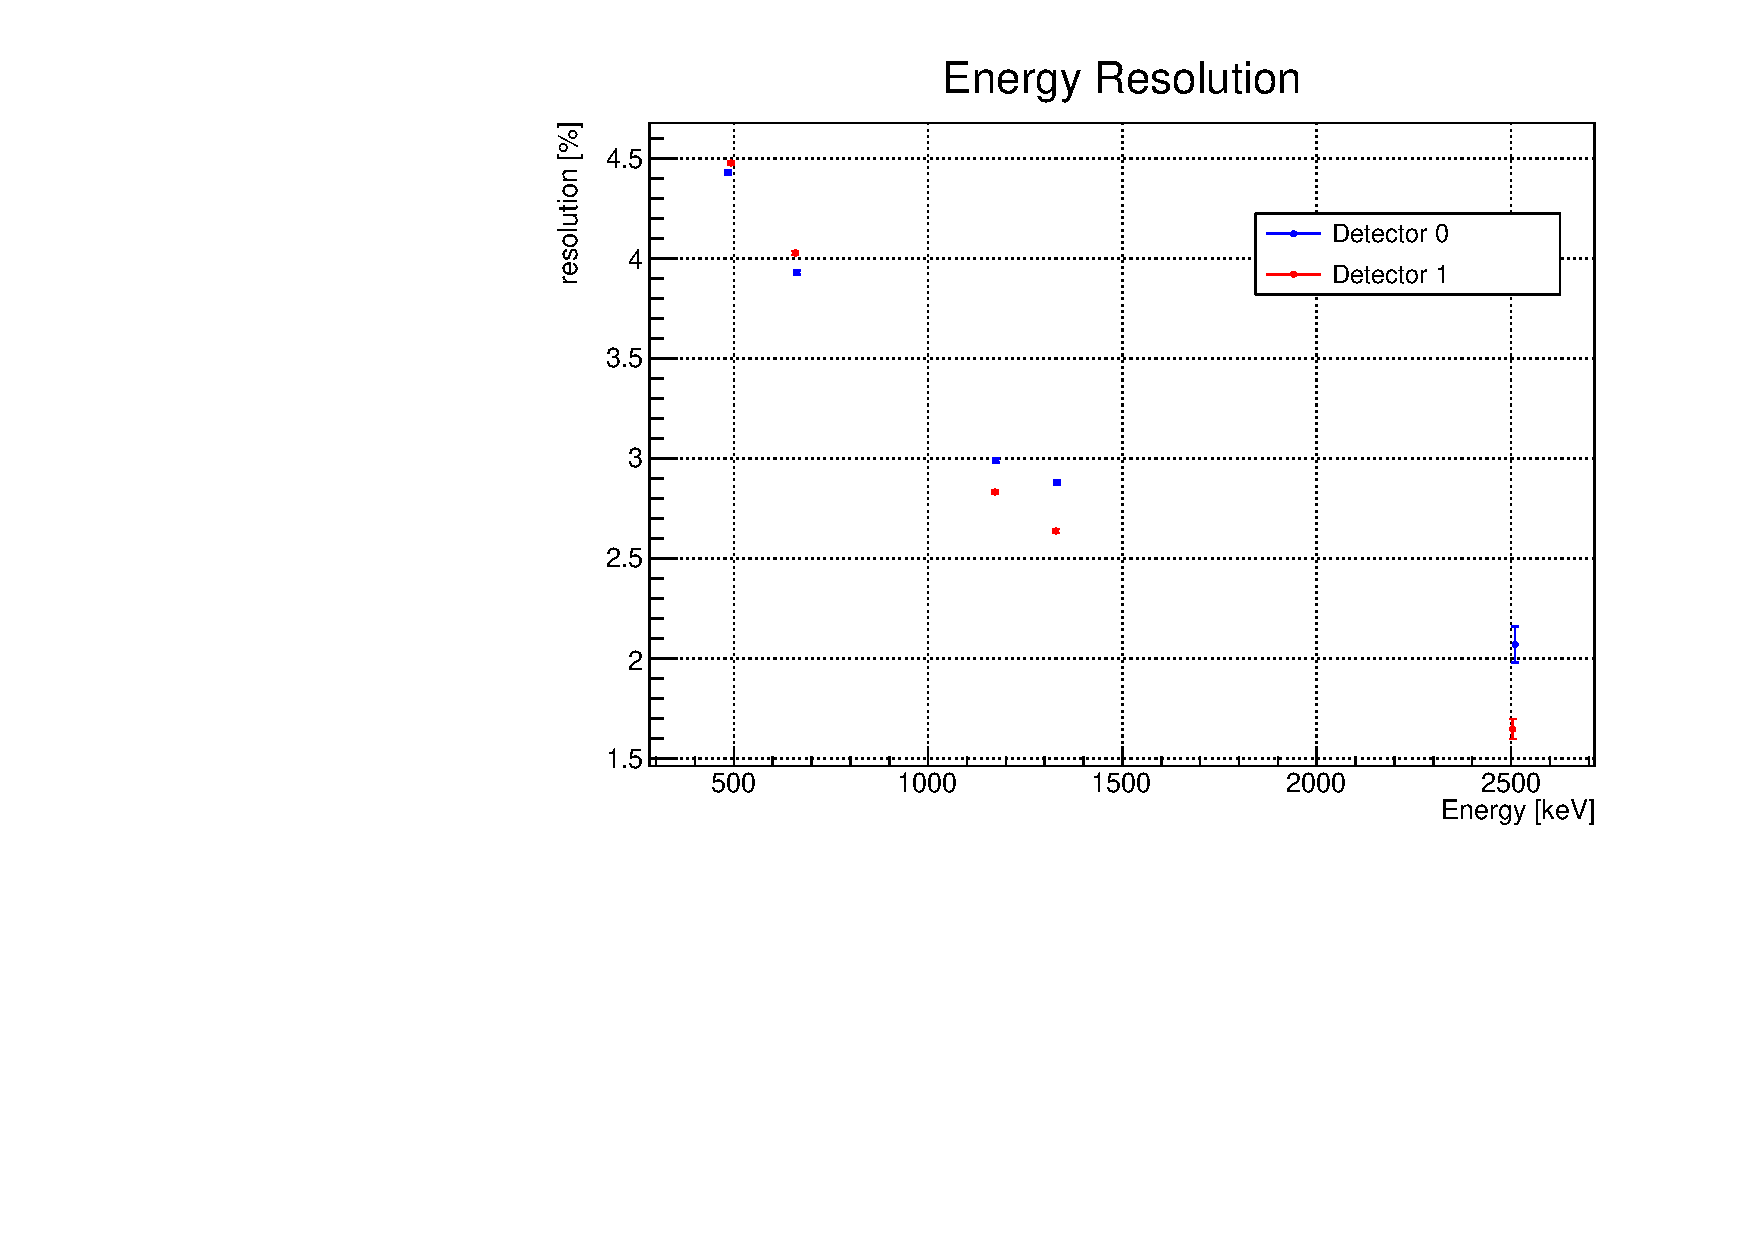
\includegraphics[scale=0.5]{Images/analysis/resolution/res.pdf}
    \caption{Energy resolution of the detectors, with detector 0 in blue and detector 1 in red.}
    \label{fig:res}
\end{figure}

\begin{table}[h]
    \begin{subtable}
        \centering
        \begin{tabular}{|c|c|c|c|}
         \hline
        E [keV] & $\sigma_{E} $ [keV] & res [\%] &$\sigma_{res}$ [\%]  \\
        \hline
        485.34 & 0.02 & 4.43 & 0.01 \\
        661.65 & 0.02 & 3.93 & 0.01 \\
        1173.84 &0.04& 2.99 & 0.01\\
        1331.70 & 0.04&2.88& 0.01\\
        2510.5 & 0.9&2.07& 0.09\\
        \hline
        \end{tabular}
    \end{subtable}
    \qquad
    \qquad
    \qquad
    \begin{subtable}
        \centering
        \begin{tabular}{|c|c|c|c|}
          \hline
        E [keV] & $\sigma_{E} $ [keV] & res [\%] &$\sigma_{res}$ [\%]  \\
        \hline
        493.29 & 0.02 &4.47 & 0.01 \\
        661.68 & 0.02 & 4.02 & 0.01 \\
        1173.64 &0.03& 2.83 & 0.01\\
        1332.17 & 0.03&2.63& 0.01\\
        2506.8 & 0.5&1.64& 0.05\\
        \hline
        \end{tabular}
     \end{subtable}
     \caption{Values of resolution at different energies for detector 0 and 1 respectively.}
     \label{tab:res}
\end{table}

We can then fit the values for the resolution an FWHM to some commonly used functions \cite{gilmore_2008}, shown respectively in the first and second table of tab. \ref{table:Funzioni}.
The results of said fits are shown in fig. \ref{fig:resolution} for the resolution and in fig. \ref{fig:FWHM} for the FWHM, while the values of the parameters of the fit are shown in tab. \ref{table:fit_res0}-\ref{table:fit_FWHM1}.

\begin{table}[h]
    \begin{subtable}
        \centering
        \begin{tabular}{|c|c|}
        \hline
        \multicolumn{2}{|c|}{Function to fit the resolution}\\
        \hline
        F1 & $ res = \frac{a}{E} + b$\\
        F2 & $ res = \frac{a}{E} + b + c \cdot E $ \\
        F3 & $ res = \frac{a}{E} + \frac{b}{E^{3/2}}$\\
        F4 & $ res = \sqrt{\frac{a^2}{E^2}+\frac{b^2}{E}}$\\
        F5 & $ res = \sqrt{\frac{a^2}{E^2}+\frac{b^2}{E}+c^2}$\\
        \hline
        \end{tabular}
    \end{subtable}
    \qquad
    \qquad
    \qquad
    \begin{subtable}
        \centering
        \begin{tabular}{|c|c|}
        \hline
        \multicolumn{2}{|c|}{Functions to fit the FWHM}\\
        \hline
        G1 & $ FWHM = a + b \cdot E$\\
        G2 & $ FWHM = a+ b \cdot E + c \cdot E^{2} $ \\
        G3 & $ FWHM = a + \frac{b}{\sqrt{E}}$\\
        G4 & $ FWHM = \sqrt{a^2+b^2 E} $\\
        G5 & $ FWHM = \sqrt{a^2+b^2E+c^2E^2}$\\
       \hline
        \end{tabular}
     \end{subtable}
     \caption{Functions used for fitting the energy resolution and the FWHM, respectively.}
     \label{table:Funzioni}
\end{table}

\begin{figure}[H]
	\begin{minipage}[c]{0.5\linewidth}
	\subfloat[][Channel 0.]{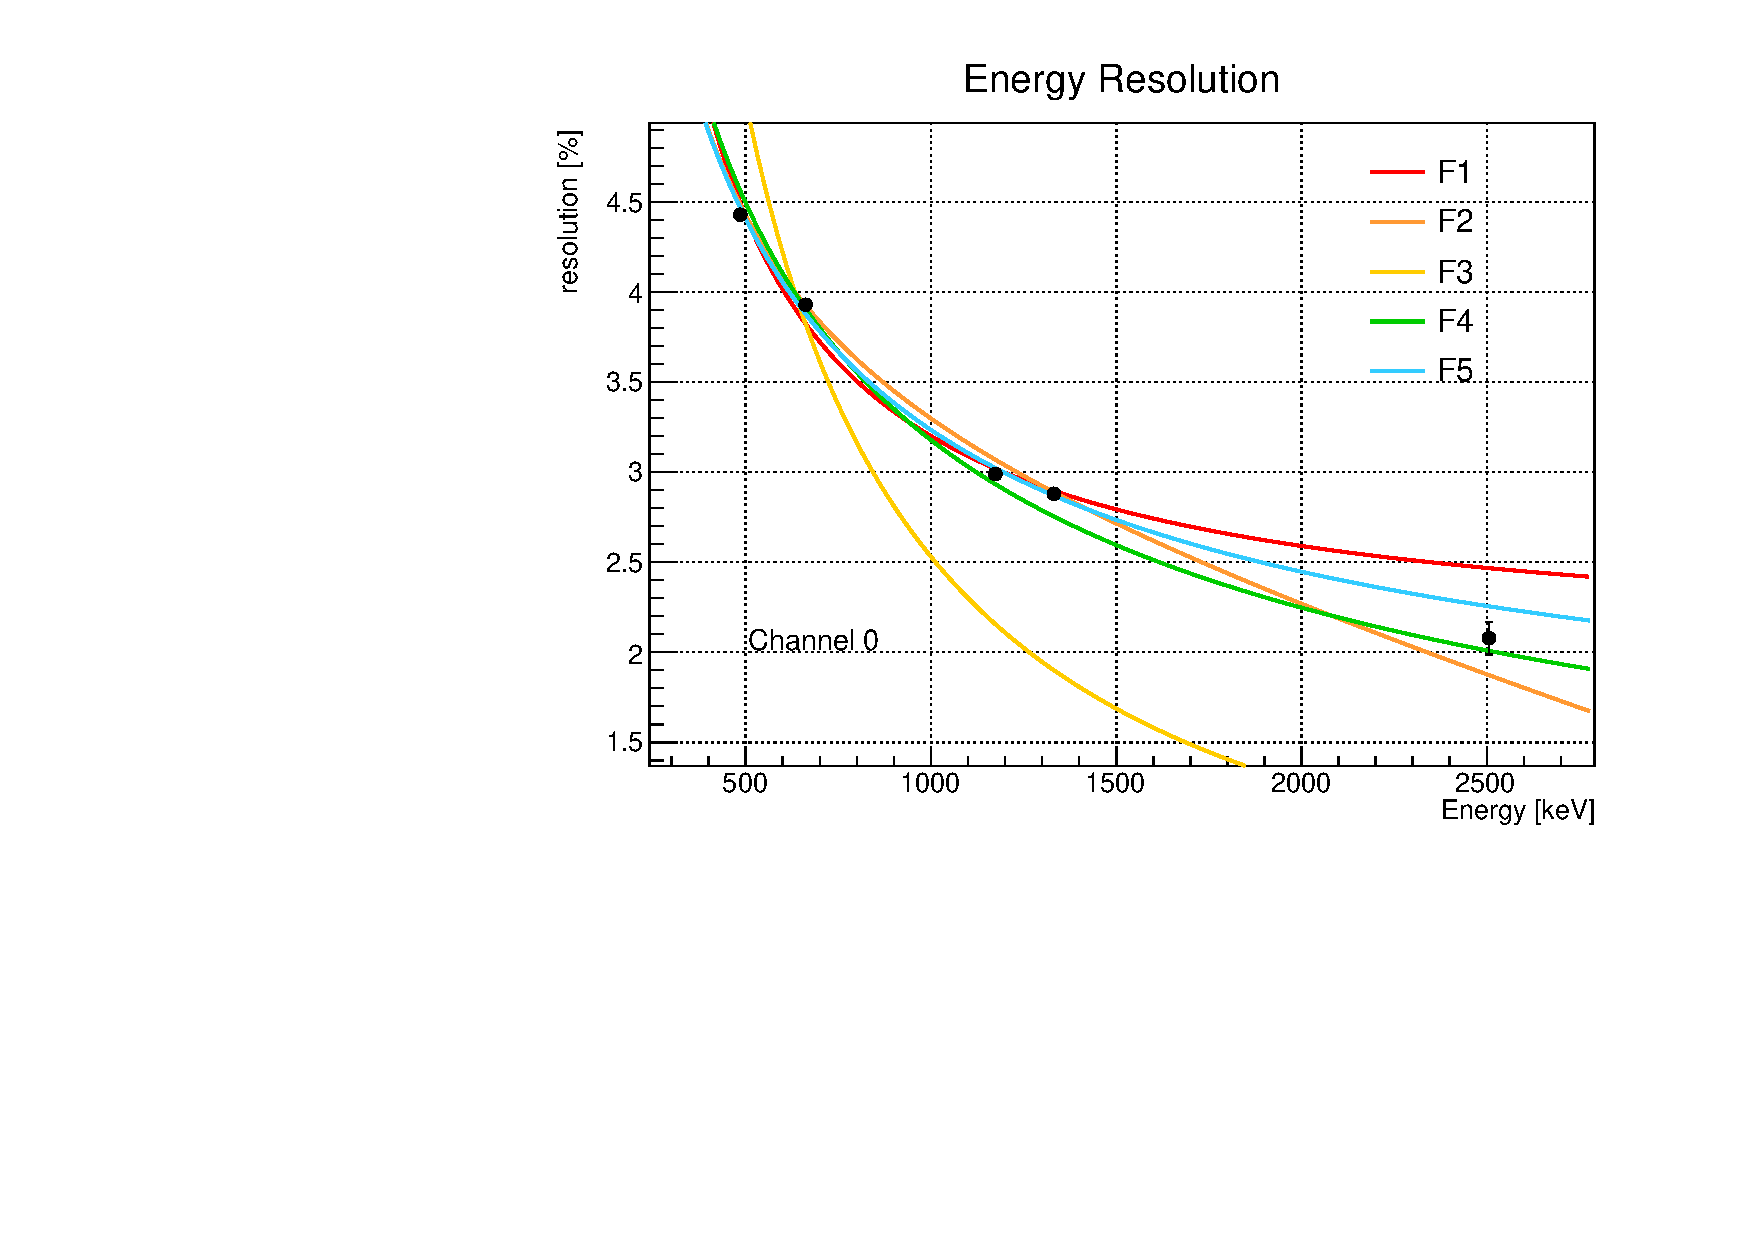
\includegraphics[width=0.9\textwidth]{Images/analysis/resolution/res0_fit.pdf} \label{fig:res0} }
	\end{minipage}
	\begin{minipage}[]{0.5\linewidth}
	\centering
	\subfloat[][Channel 1.]{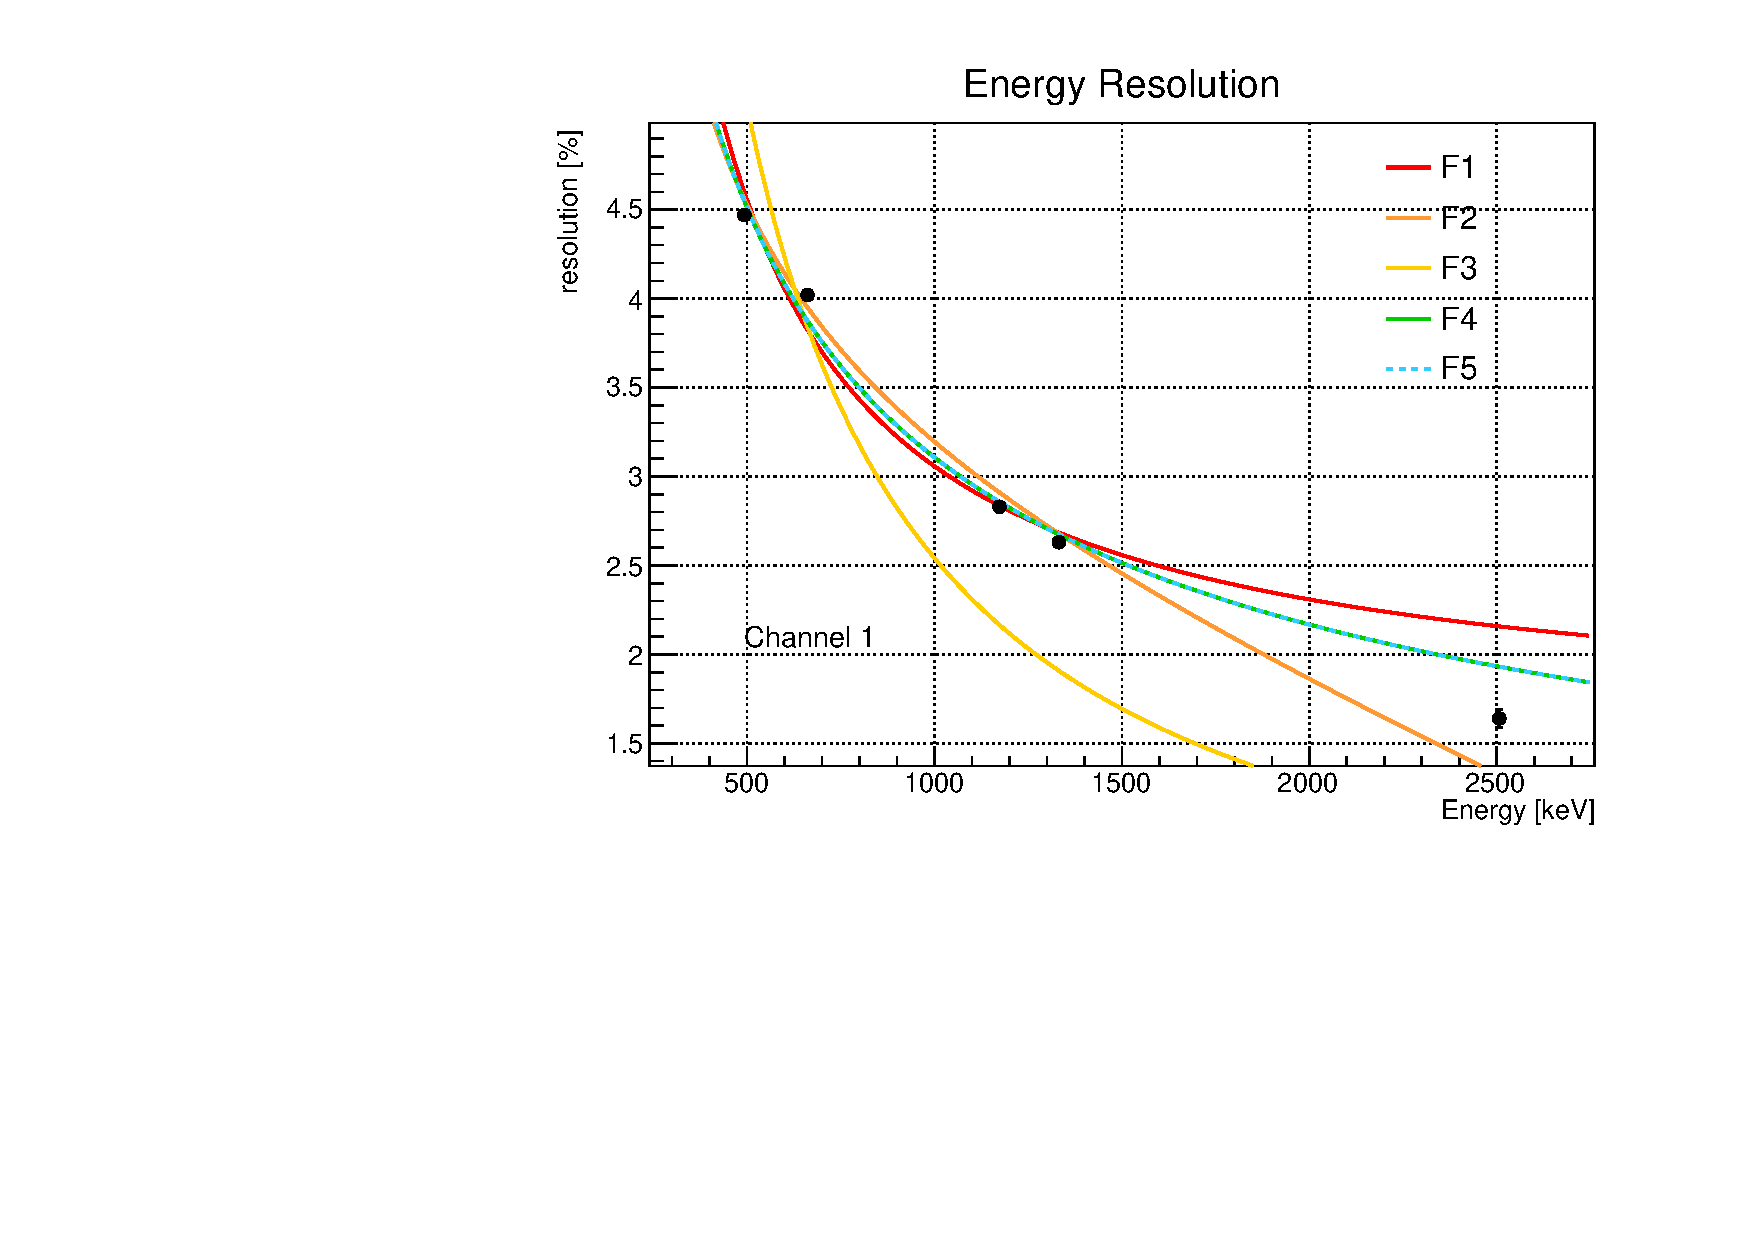
\includegraphics[width=0.9\textwidth]{Images/analysis/resolution/res1_fit.pdf}  \label{fig:res1} }
	\end{minipage}
	\caption{Fit of the energy resolution through the functions in the first table of tab.\ref{table:Funzioni}.}
    \label{fig:resolution}
	\end{figure}

\begin{figure}[H]
	\begin{minipage}[c]{0.5\linewidth}
	\subfloat[][Channel 0.]{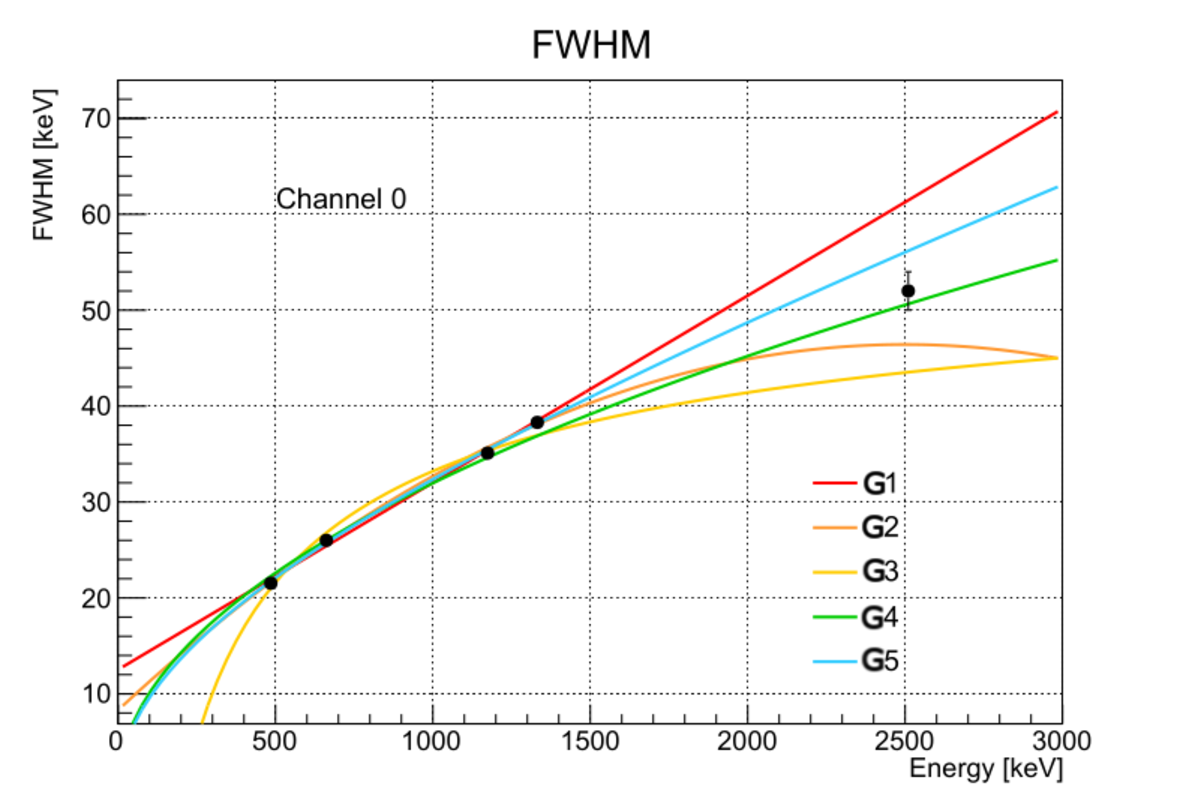
\includegraphics[width=0.9\textwidth]{Images/analysis/resolution/FWHM0.pdf} \label{fig:FWHM0} }
	\end{minipage}
	\begin{minipage}[]{0.5\linewidth}
	\centering
	\subfloat[][Channel 1.]{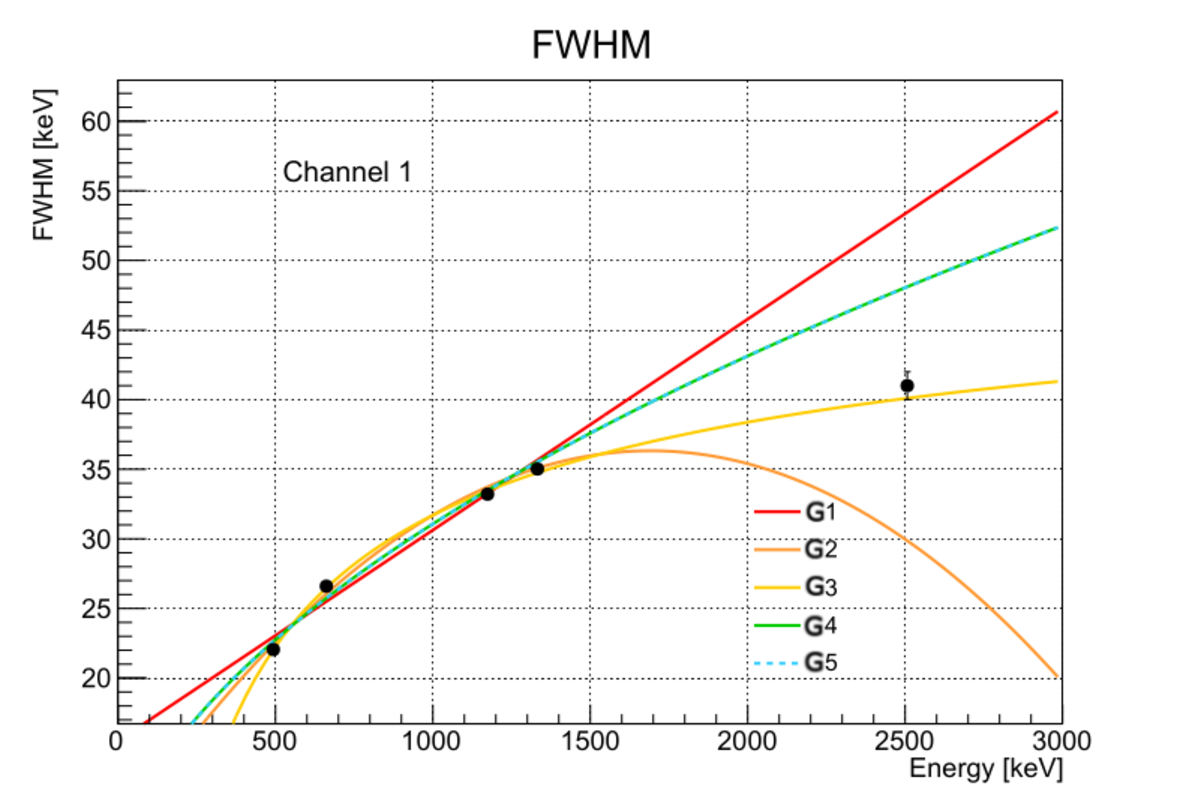
\includegraphics[width=0.9\textwidth]{Images/analysis/resolution/FWHM1.pdf}  \label{fig:FWHM1} }
	\end{minipage}
	\caption{Fit of the FWHM through the functions in the second table of tab.\ref{table:Funzioni}.}
    \label{fig:FWHM}
	\end{figure}

\begin{table}[ht]
    \centering
    \begin{tabular}{|c|c|c|c|c|}
    \hline
     & a & b & c & $\chi /dof$  \\
    \hline
    F1 & $(1220 \pm 9)$ keV & $(1.98 \pm 0.01)$ & - & 183.6/3 \\
    F2 & $(8.2 \pm 0.4) \times 10^2$ keV & $(3.1 \pm 0.1)$ & $(-0.62 \pm 0.05)10^{-3}$ keV$^{-1}$ & 52.01/2 \\
    F3 & $(2 \pm 1) \times 10^3$ keV & $(1 \pm 1)10^3$ keV$^{3/2}$ & - & 22950/3 \\
    F4 & $(0.0 \pm 0.6)$ keV & $(100.5 \pm 0.1)$ keV$^{1/2}$ & - & 370.5/3 \\
    F5 & $(0 \pm 2)$ keV & $(94.6 \pm 0.4)$ keV$^{1/2}$ & $(1.23 \pm 0.03)$ & 56.34/2 \\
    \hline
    \end{tabular}
    \caption{Parameters of the functions fitting energy resolution for detector 0.}
    \label{table:fit_res0}
\end{table}

\begin{table}[ht]
    \centering
    \begin{tabular}{|c|c|c|c|c|}
    \hline
     & a & b & c & $\chi /dof$  \\
    \hline
    F1 & $(15.0 \pm 0.1) \times 10^2$ keV & $(1.56 \pm 0.01)$ & - & 681.90/3 \\
    F2 & $(8.9 \pm 0.3) \times 10^2$ keV & $(3.2 \pm 0.1)$ & $(-0.89 \pm 0.04) \times 10^{-3}$ keV$^{-1}$ & 209.4/2 \\
    F3 & $(2 \pm 0.5) \times 10^3$ keV & $(0.8 \pm 0.5)10^4$ keV$^{3/2}$ & - & 14760/3 \\
    F4 & $(7.2 \pm 0.4) \times 10^2$ keV & $(95.6 \pm 0.4)$ keV$^{1/2}$ & - & 334.8/3 \\
    F5 & $(7.2 \pm 0.3) \times 10^2$ keV & $(94.6 \pm 0.4)$ keV$^{1/2}$ & $(0.00 \pm 0.01)$ & 334.8/2\\
    \hline
    \end{tabular}
    \caption{Parameters of the functions fitting energy resolution for detector 1, note that the results for F4 and F5 are the same.}
    \label{table:fit_res1}
\end{table}

\begin{table}[ht]
    \centering
    \begin{tabular}{|c|c|c|c|c|}
    \hline
     & a & b & c & $\chi /dof$  \\
    \hline
    G1 & $(12.52 \pm 0.08)$ keV & $(0.0195 \pm 0.0001)$ & - & 251.6/3 \\
    G2 & $(8.3 \pm 0.3)$ keV & $(0.0305 \pm 0.0008)$ & $(-6.1 \pm 0.5) \times 10^{-6}$ keV $^{-1}$ & 68.81/2 \\
    G3 & $(61.2 \pm 0.2)$ keV & $(-885 \pm 5)$ keV$^{3/2}$ & - & 560.8/3 \\
    G4 & $(0.00 \pm 0.01)$ keV & $(1.011 \pm 0.001)$ keV$^{1/2}$ & - & 440.1/3 \\
    G5 & $(0.000 \pm 0.004)$ keV & $(0.953 \pm 0.003)$ keV$^{1/2}$ & $(0.0118 \pm 0.0003)$ & 71.16/2 \\
    \hline
    \end{tabular}
    \caption{Parameters of the functions fitting FWHM for detector 0.}
    \label{table:fit_FWHM0}
\end{table}

\begin{table}[H]
    \centering
    \begin{tabular}{|c|c|c|c|c|}
    \hline
     & a & b & c & $\chi /dof$  \\
    \hline
    G1 & $(15.48 \pm 0.07)$ keV & $(0.01515 \pm 0.00009)$ & - & 1480/3 \\
    G2 & $(8.6 \pm 0.2)$ keV & $(0.0328 \pm 0.0006)$ & $(-9.7 \pm 0.3) \times 10^{-6}$ keV$^{-1}$ & 450.7/2 \\
    G3 & $(54.5 \pm 0.2)$ keV & $(-721 \pm 4)$ keV$^{3/2}$ & - & 31/3 \\
    G4 & $(8.4 \pm 0.2) \times 10^2$ keV & $(0.946 \pm 0.003)$ keV$^{1/2}$ & - & 773.9/3 \\
    G5 & $(8.4 \pm 0.2) \times 10^2$ keV & $(0.946 \pm 0.003)$ keV$^{1/2}$ & $(0.00 \pm 0.02)10^{-3}$ & 773.9/2\\
    \hline
    \end{tabular}
    \caption{Parameters of the functions fitting FWHM for detector 1, note that the results for G4 and G5 are the same.}
    \label{table:fit_FWHM1}
\end{table}